%  Created by Matthew Rásó-Barnett on 2009-08-10	
\documentclass[11pt,a4paper,oneside]{article}

% Setup for fullpage use - Reduces the margins at the sides
\usepackage{fullpage}

% -------------------------------------

% More symbols
\usepackage{amssymb}
\usepackage[intlimits]{amsmath}
\usepackage{latexsym}

\usepackage[parfill]{parskip}  % Activate to begin paragraphs with an empty line
\usepackage{epstopdf}
\usepackage{mathrsfs} % mathrsfs is for producing the curly H for Hilbert space
\DeclareMathAlphabet{\mathpzc}{OT1}{pzc}{m}{it} % This is to define another curly type of font called with \mathpzc{ }
\usepackage{dsfont} % For identity symbol

\usepackage[pdftex]{graphicx}
\usepackage[usenames,dvipsnames]{color}

% -------------------------------------

% For Source code, use the listings environment
\usepackage{listings}
\usepackage{courier}
\lstset{
	language=C,
	basicstyle=\scriptsize\ttfamily, 
	numberstyle=\tiny,          
	numbersep=5pt,              
	tabsize=2,                  
	extendedchars=true,         
	breaklines=true,            
	keywordstyle=\color{red},
	stringstyle=\color{white}\ttfamily, 
	showspaces=false,           
	showtabs=false,             
	xleftmargin=17pt,
	framexleftmargin=17pt,
	framexrightmargin=5pt,
	framexbottommargin=4pt,
	%backgroundcolor=\color{lightgray},
	showstringspaces=false,          
	keywordstyle=\color{blue},
	commentstyle=\color{OliveGreen},
	stringstyle=\color{red},
	numbers=left,
	numberstyle=\tiny,
	numbersep=5pt,
	breaklines=true,
	emph={label}
}
\lstloadlanguages{% Check Dokumentation for further languages ...
	%C
	C++
	%XML
	%HTML
	%Java
}
%\DeclareCaptionFont{blue}{\color{blue}} 
%\captionsetup[lstlisting]{singlelinecheck=false, labelfont={blue}, textfont={blue}}
\usepackage{caption}
\DeclareCaptionFont{white}{\color{white}}
\DeclareCaptionFormat{listing}{\colorbox[cmyk]{0.43, 0.35, 0.35,0.01}{\parbox{\textwidth}{\hspace{15pt}#1#2#3}}}
\captionsetup[lstlisting]{format=listing,labelfont=white,textfont=white, singlelinecheck=false, margin=0pt, font={bf,scriptsize}}

% -------------------------------------

% For Floats
\usepackage{float}

% New float for source code examples
\floatstyle{plain} 
\newfloat{sourcecode}{!htb}{}{}
\floatname{sourcecode} 

% Multipart figures
\usepackage{subfig}

% -------------------------------------

\DeclareGraphicsExtensions{.pdf, .jpg, .png}

\begin{document}



\section*{Neutron Loss at the Boundary for the Case of $E > V_{f}$}

James Sinclair and I have been thinking about an aspect of how we initialise the neutron velocity distribution in our simulations. If, for example, we take a $v^{2}$ distribution of velocities we need to choose a range of velocities to pick between, which usually results in the situation shown in figure \ref{fig:velocitydistribution}. Here we pick velocities between zero and a velocity equivalent to the Fermi potential of our wall material - thus we are assuming that every neutron with an $E_{\perp}$ greater than $V_{F}$ will be lost. However, a more realistic distribution, roughly like that in figure \ref{fig:velocitydistribution2} doesn't have this hard cut-off at the equivalent $V_{F}$, but instead has a decreasing tail. 

\begin{figure}[!htbp] 
\centering 
\subfloat[$v^{2}$ with hard cutoff] {\label{fig:velocitydistribution} 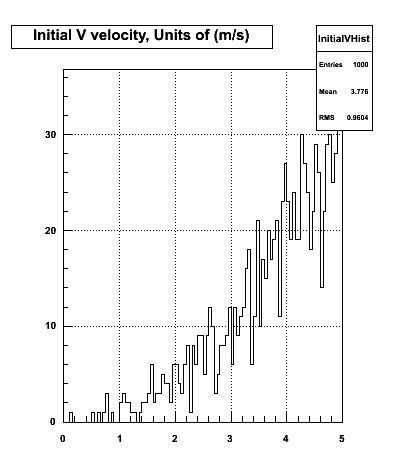
\includegraphics[width=0.3\textwidth] {figures/initialspectrum}} \hspace{2mm} 
\subfloat[$v^{2}$ with tail] {\label{fig:velocitydistribution2} 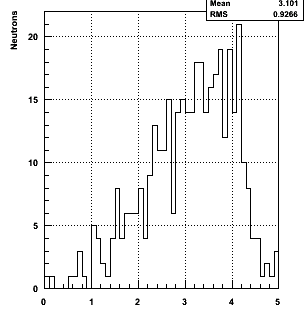
\includegraphics[width=0.3\textwidth] {figures/initialspectrum2}} \hspace{2mm}
\caption{Current and desired initial UCN velocity distributions} 
\label{fig:distributions} 
\end{figure}

My understanding for this tail is that 1.) Neutrons with a kinetic energy above, but close to the Fermi potential will still be reflected at shallow angles, so that $E_{\perp} < V_{F}$; 2.) Neutrons with $E_{\perp} > V_{F}$ can also still be reflected with a vanishingly small probability the further you go above the Fermi potential. 

It is the neutrons in the second case that James and I were thinking about as we thought about how we could treat them in our simulations. The quantum mechanical expression for the reflection/transmision probability from a potential step can of course be used to calculate how many will be reflected/transmitted with $E_{\perp} > V_{F}$, however we were thinking about how we would calculate the probability of loss through absorption/upscattering for this case, since the usual loss-probability equation, \ref{eqn:angle-averagedlossprobability}, derived using the complex potential method, doesn't apply to this case.  

\begin{equation}
\mu(E, \theta) = 1 - |R|^{2} = 2f \left( \frac{E\cos^{2}\theta}{V-E\cos^{2}\theta} \right)^{1/2}
\label{eqn:angle-averagedlossprobability}
\end{equation}

Losses through absorption/upscattering are probably small in this case, and overshadowed by the number being transmitted into the boundary (and perhaps captured or inelastically scattered by the nuclei later), but we are just thinking about how you would calculate the probability of loss, and whether this would have an additional contribution to producing this tail in the velocity distribution above the Fermi potential? 

Would we go back to the equation for $|R|^{2}$ in terms of $U = V - iW$ and re-arrange this into an equivalent form as before $|R|^{2} \equiv 1 - \mu(E,\theta)$, without this time assuming $E_{\perp} < V$, or do we need to take a different approach here?

I find it difficult to think of nuclear absorption in the context of quantum mechanical reflection/transmission by 1D potentials. In the usual case where $E_{\perp} < V$, the wavefunction decays exponentially into the boundary, since the wave-vector in this region is imaginary - and we use this idea, when we introduce a complex potential, $U$, to give a description of the loss by absorption. Also, in the document you sent me around christmas time regarding the use of the complex potential $W$, you said that, 

\begin{quote}
When there is slow neutron density in the vicinity of a nucleus there is a proportionate but higher density of neutron inside the attractive nuclear well. The velocity (energy) of the neutron inside the well is completely dominated by the depth of the nuclear well order 10s of MeV. The energy of a neutron approaching the nucleus at $<$ 0.01 eV has a completely negligible effect on the neutron energy and reaction rate (capture rate) when it is inside the nucleus. So a given species of nucleus, eg 3He has a given reaction rate proportional to the local
neutron density but independent of the slow neutron velocity.
\end{quote}

So if the absorption rate is only proportional to the local neutron density, in the case that $E_{\perp} > V$, wouldn't the reaction rate decrease to zero as the wavefunction is no longer inside the potential barrier in the reflected region, and instead only neutrons transmitted into the boundary region would be able to be captured by nuclei?



Thanks.

\end{document}